% !TEX TS-program = pdflatex
% !TEX encoding = UTF-8 Unicode

% This is a simple template for a LaTeX document using the "article" class.
% See "book", "report", "letter" for other types of document.

\documentclass[8pt]{article} % use larger type; default would be 10pt

\usepackage[utf8]{inputenc} % set input encoding (not needed with XeLaTeX)
\usepackage{bchart}
\usepackage{longtable}
\usepackage{pgfgantt}
\usepackage{calendar} % Use the calendar.sty style


%%% Examples of Article customizations
% These packages are optional, depending whether you want the features they provide.
% See the LaTeX Companion or other references for full information.

\usepackage{textcomp}
%\usepackage{hyperref}

%%% PAGE DIMENSIONS
\usepackage{geometry} % to change the page dimensions
\geometry{a4paper} % or letterpaper (US) or a5paper or....
% \geometry{margin=2in} % for example, change the margins to 2 inches all round
% \geometry{landscape} % set up the page for landscape
%   read geometry.pdf for detailed page layout information

\usepackage{graphicx} % support the \includegraphics command and options

% \usepackage[parfill]{parskip} % Activate to begin paragraphs with an empty line rather than an indent

%%% PACKAGES
\usepackage{booktabs} % for much better looking tables
\usepackage{array} % for better arrays (eg matrices) in maths
\usepackage{paralist} % very flexible & customisable lists (eg. enumerate/itemize, etc.)
\usepackage{verbatim} % adds environment for commenting out blocks of text & for better verbatim
\usepackage{subfig} % make it possible to include more than one captioned figure/table in a single float
% These packages are all incorporated in the memoir class to one degree or another...

%%% HEADERS & FOOTERS
\usepackage{fancyhdr} % This should be set AFTER setting up the page geometry
\pagestyle{fancy} % options: empty , plain , fancy
\renewcommand{\headrulewidth}{0pt} % customise the layout...
\lhead{}\chead{}\rhead{}
\lfoot{}\cfoot{\thepage}\rfoot{}

%%% SECTION TITLE APPEARANCE
\usepackage{sectsty}
\allsectionsfont{\sffamily\mdseries\upshape} % (See the fntguide.pdf for font help)
% (This matches ConTeXt defaults)

%%% ToC (table of contents) APPEARANCE
\usepackage[nottoc,notlof,notlot]{tocbibind} % Put the bibliography in the ToC
\usepackage[titles,subfigure]{tocloft} % Alter the style of the Table of Contents
\renewcommand{\cftsecfont}{\rmfamily\mdseries\upshape}
\renewcommand{\cftsecpagefont}{\rmfamily\mdseries\upshape} % No bold!

%%% END Article customizations

%%% The "real" document content comes below...

\title{Management overview}
\author{\copyright Frederic Kerdraon}
%\date{} % Activate to display a given date or no date (if empty),
         % otherwise the current date is printed 

\begin{document}
\maketitle
\tableofcontents
\section{Introduction}

This document summurizes all the important informations necessary to facilitate things and remove a lot of stress. It's been put together thanks to \LaTeX. This is designed to help make optimal decisions for a not so short lifetime.

Ce n'est pas parceque les choses sont difficiles que nous n'osons pas, c'est parceque nous n'osons pas qu'elles sont difficiles.
%\makebox[2\width]{hello}
\texteuro

\section{Organisation}
\subsection{Karima weekly call}

\section{Communication}

\subsection{Karima}
	Me laisser aider sur la methodo et l'orga\\
	Me laisser un acces a distance\\
	Si le systeme marche, ca ne sera que du bonheur pour toi\\
	J'ai une vie personelle\\
\subsection{Aymeric}
	Fermer sa gueule\\
\subsection{Julien}
	M'apprendre Murex\\

\section{Calendars}
\subsection{Yearly calendar}

\begin{calendar}{\hsize}
 
%----------------------------------------------------------------------------------------
%	BLANK DAYS BEFORE THE BEGINNING OF THE CALENDAR
%----------------------------------------------------------------------------------------

% This part is very finicky. It defines the number of blank days at the beginning of the calendar before the first of the month starts. If you need this to be more than 4 (i.e. the first starts on a Friday or Saturday in a 31 day month), then you have two options: 
% 1) You can uncomment another one or two \BlankDay's below which will make a new week (6 total) which makes the calendar too big for one page, remedy this by decreasing the size of each day by replacing 2.5cm below with a smaller number. 
% 2) Make the spill-over days start at the top left of the calendar (i.e. the calendar starts with 31 then a few days blank then 1, 2, 3, etc). The second option can be configured by uncommenting the below:

%\setcounter{calendardate}{31} % Begin the count with 31 so the top left day is 31; this can be changed to 29 or 30 as required
%\day{}{\vspace{2.5cm}} % 31 - add another line identical to this if starting at 30 or earlier

% You will need to comment out the 31 in the NUMBERED DAYS AND CALENDAR CONTENT section below for this as well as commenting out one of the \BlankDay's below. Play around with it and you will get it.

\BlankDay
\BlankDay
%\BlankDay
%\BlankDay
%\BlankDay
%\BlankDay

%----------------------------------------------------------------------------------------
%	NUMBERED DAYS AND CALENDAR CONTENT
%----------------------------------------------------------------------------------------

% These are the numbered days in the template - if there are less than 31 days simply comment out the bottom lines.

% \vspace{2.5cm} is only there to provide an even look to the calendar where each day is 2.5cm tall, it can be changed or removed to automatically adjust to the day in the week with the most content

\setcounter{calendardate}{1} % Start the date counter at 1

\day{Work}{10am Meeting with Boss \\[6pt] 12pm Meeting with Group} % 1 - Example of content
\day{}{\vspace{2.5cm}} % 2 
\day{}{\vspace{2.5cm}} % 3
\day{}{\vspace{2.5cm}} % 4
\day{}{\vspace{2.5cm}} % 5
\day{}{\vspace{2.5cm}} % 6
\day{}{\vspace{2.5cm}} % 7
\day{}{\vspace{2.5cm}} % 8
\day{}{\vspace{2.5cm}} % 9
\day{}{\vspace{2.5cm}} % 10
\day{}{\vspace{2.5cm}} % 11
\day{}{\vspace{2.5cm}} % 12
\day{}{\vspace{2.5cm}} % 13
\day{}{\vspace{2.5cm}} % 14
\day{}{\vspace{2.5cm}} % 15
\day{}{\vspace{2.5cm}} % 16
\day{}{\vspace{2.5cm}} % 17
\day{}{\vspace{2.5cm}} % 18
\day{}{\vspace{2.5cm}} % 19
\day{}{\vspace{2.5cm}} % 20 
\day{}{\vspace{2.5cm}} % 21
\day{}{\vspace{2.5cm}} % 22
\day{}{\vspace{2.5cm}} % 23
\day{}{\vspace{2.5cm}} % 24
\day{}{\vspace{2.5cm}} % 25
\day{}{\vspace{2.5cm}} % 26
\day{}{\vspace{2.5cm}} % 27
\day{}{\vspace{2.5cm}} % 28
\day{}{\vspace{2.5cm}} % 29 
\day{}{\vspace{2.5cm}} % 30 
\day{}{\vspace{2.5cm}} % 31

% Un-comment the \BlankDay below if the bottom line of the calendar is missing
%\BlankDay

% Un-comment to start counting again after 31
%\setcounter{calendardate}{1}
%\day{}{\vspace{2.5cm}} % 1
%\day{}{\vspace{2.5cm}} % 2
%\day{}{\vspace{2.5cm}} % 3

%----------------------------------------------------------------------------------------

\finishCalendar
\end{calendar}

\subsection{Weekly calendar}
\begin{calendar}{\hsize}

%----------------------------------------------------------------------------------------
%	FIRST DAY
%----------------------------------------------------------------------------------------

\day{}{\textbf{9am-5pm} \daysep Work at McDonald's} % By default all daily events are centered in the box, in order to bring them up use \vspace{2cm} after the event text; you may need to change the 2cm

%----------------------------------------------------------------------------------------
%	SECOND DAY
%----------------------------------------------------------------------------------------

\day{}{
\textbf{9am-10am} \daysep BIOSCI101 - BLT100 \\[3pt]
\textbf{10am-11am} \daysep BIOSCI 104 - LLT \\[3pt]
%\textbf{11am-12pm} \daysep No Lecture \\[3pt]
\textbf{12pm-1pm} \daysep BIOSCI105 - BLT204 \\[3pt]
%\textbf{1pm-2pm} \daysep No Lecture \\[3pt]
\textbf{2pm-5pm} \daysep BIOSCI101 Laboratory \\[3pt]
%\textbf{3pm-4pm} \daysep BIOSCI101 Laboratory \\[3pt]
%\textbf{4pm-5pm} \daysep BIOSCI101 Laboratory
} 

%----------------------------------------------------------------------------------------
%	THIRD DAY
%----------------------------------------------------------------------------------------

\day{}{ % Tuesday
\textbf{9am-10am} \daysep BIOSCI101 - BLT100 \\[3pt]
\textbf{10am-11am} \daysep BIOSCI 104 - LLT \\[3pt]
%\textbf{11am-12pm} \daysep No Lecture \\[3pt]
%\textbf{12pm-1pm} \daysep No Lecture \\[3pt]
%\textbf{1pm-2pm} \daysep No Lecture \\[3pt]
\textbf{2pm-3pm} \daysep GEO101 - HSB1 \\[3pt]
%\textbf{3pm-4pm} \daysep No Lecture \\[3pt]
%\textbf{4pm-5pm} \daysep No Lecture
} 

%----------------------------------------------------------------------------------------
%	FOURTH DAY
%----------------------------------------------------------------------------------------

\day{}{ % Wednesday
%\textbf{9am-10am} \daysep No Lecture \\[3pt]
\textbf{10am-11am} \daysep BIOSCI 104 - LLT \\[3pt]
%\textbf{11am-12pm} \daysep No Lecture \\[3pt]
\textbf{12pm-1pm} \daysep BIOSCI105 - BLT204 \\[3pt]
%\textbf{1pm-2pm} \daysep No Lecture \\[3pt]
\textbf{2pm-3pm} \daysep GEO101 - HSB1 \\[3pt]
%\textbf{3pm-4pm} \daysep No Lecture \\[3pt]
%\textbf{4pm-5pm} \daysep No Lecture
} 

%----------------------------------------------------------------------------------------
%	FIFTH DAY
%----------------------------------------------------------------------------------------

\day{}{ % Thursday
%\textbf{9am-10am} \daysep No Lecture \\[3pt]
\textbf{10am-11am} \daysep BIOSCI 104 - LLT \\[3pt]
%\textbf{11am-12pm} \daysep No Lecture \\[3pt]
%\textbf{12pm-1pm} \daysep No Lecture \\[3pt]
%\textbf{1pm-2pm} \daysep No Lecture \\[3pt]
\textbf{2pm-3pm} \daysep GEO101 - HSB1 \\[3pt]
%\textbf{3pm-4pm} \daysep No Lecture \\[3pt]
%\textbf{4pm-5pm} \daysep No Lecture
} 

%----------------------------------------------------------------------------------------
%	SIXTH DAY
%----------------------------------------------------------------------------------------

\day{}{ % Friday
\textbf{9am-10am} \daysep BIOSCI101 - BLT100 \\[3pt]
\textbf{10am-11am} \daysep BIOSCI 104 - LLT \\[3pt]
%\textbf{11am-12pm} \daysep No Lecture \\[3pt]
\textbf{12pm-1pm} \daysep BIOSCI105 - BLT204 \\[3pt]
%\textbf{1pm-2pm} \daysep No Lecture \\[3pt]
%\textbf{2pm-3pm} \daysep No Lecture \\[3pt]
\textbf{3pm-4pm} \daysep GEO101 Tutorial \\ Room A \\[3pt]
%\textbf{4pm-5pm} \daysep No Lecture
} 

%----------------------------------------------------------------------------------------
%	SEVENTH DAY
%----------------------------------------------------------------------------------------

\day{}{} % Saturday

%----------------------------------------------------------------------------------------
 
\finishCalendar
\end{calendar}






\section{Checklists}
\subsection{Daily Morning}


\section{Finance}	

\subsection{Monthly summary}
Sorted by cost\\
Maturity\\
Pricing\\

\subsection{Value At Risk}

Monte carlo simulation from bionic turtle/ scilab\\
$\lim_{x \to \infty} \exp(-x) = 0$

\subsection{Sensitivities}
To be calculated : Kapital = Assets - Liabilities

\section{Projects}

plan/tasks/mgt summ/risks/charge?\\

\subsection{Deliverables}
\subsection{Document templates}
\subsection{Steps}
Inception\\
Specification\\
Clearchoice\\
External design\\
Internal design\\
Test documentation\\
Release notes\\
Post implementation review\\
Support documentation\\

\subsection{ROI}

\subsection{Budget}

%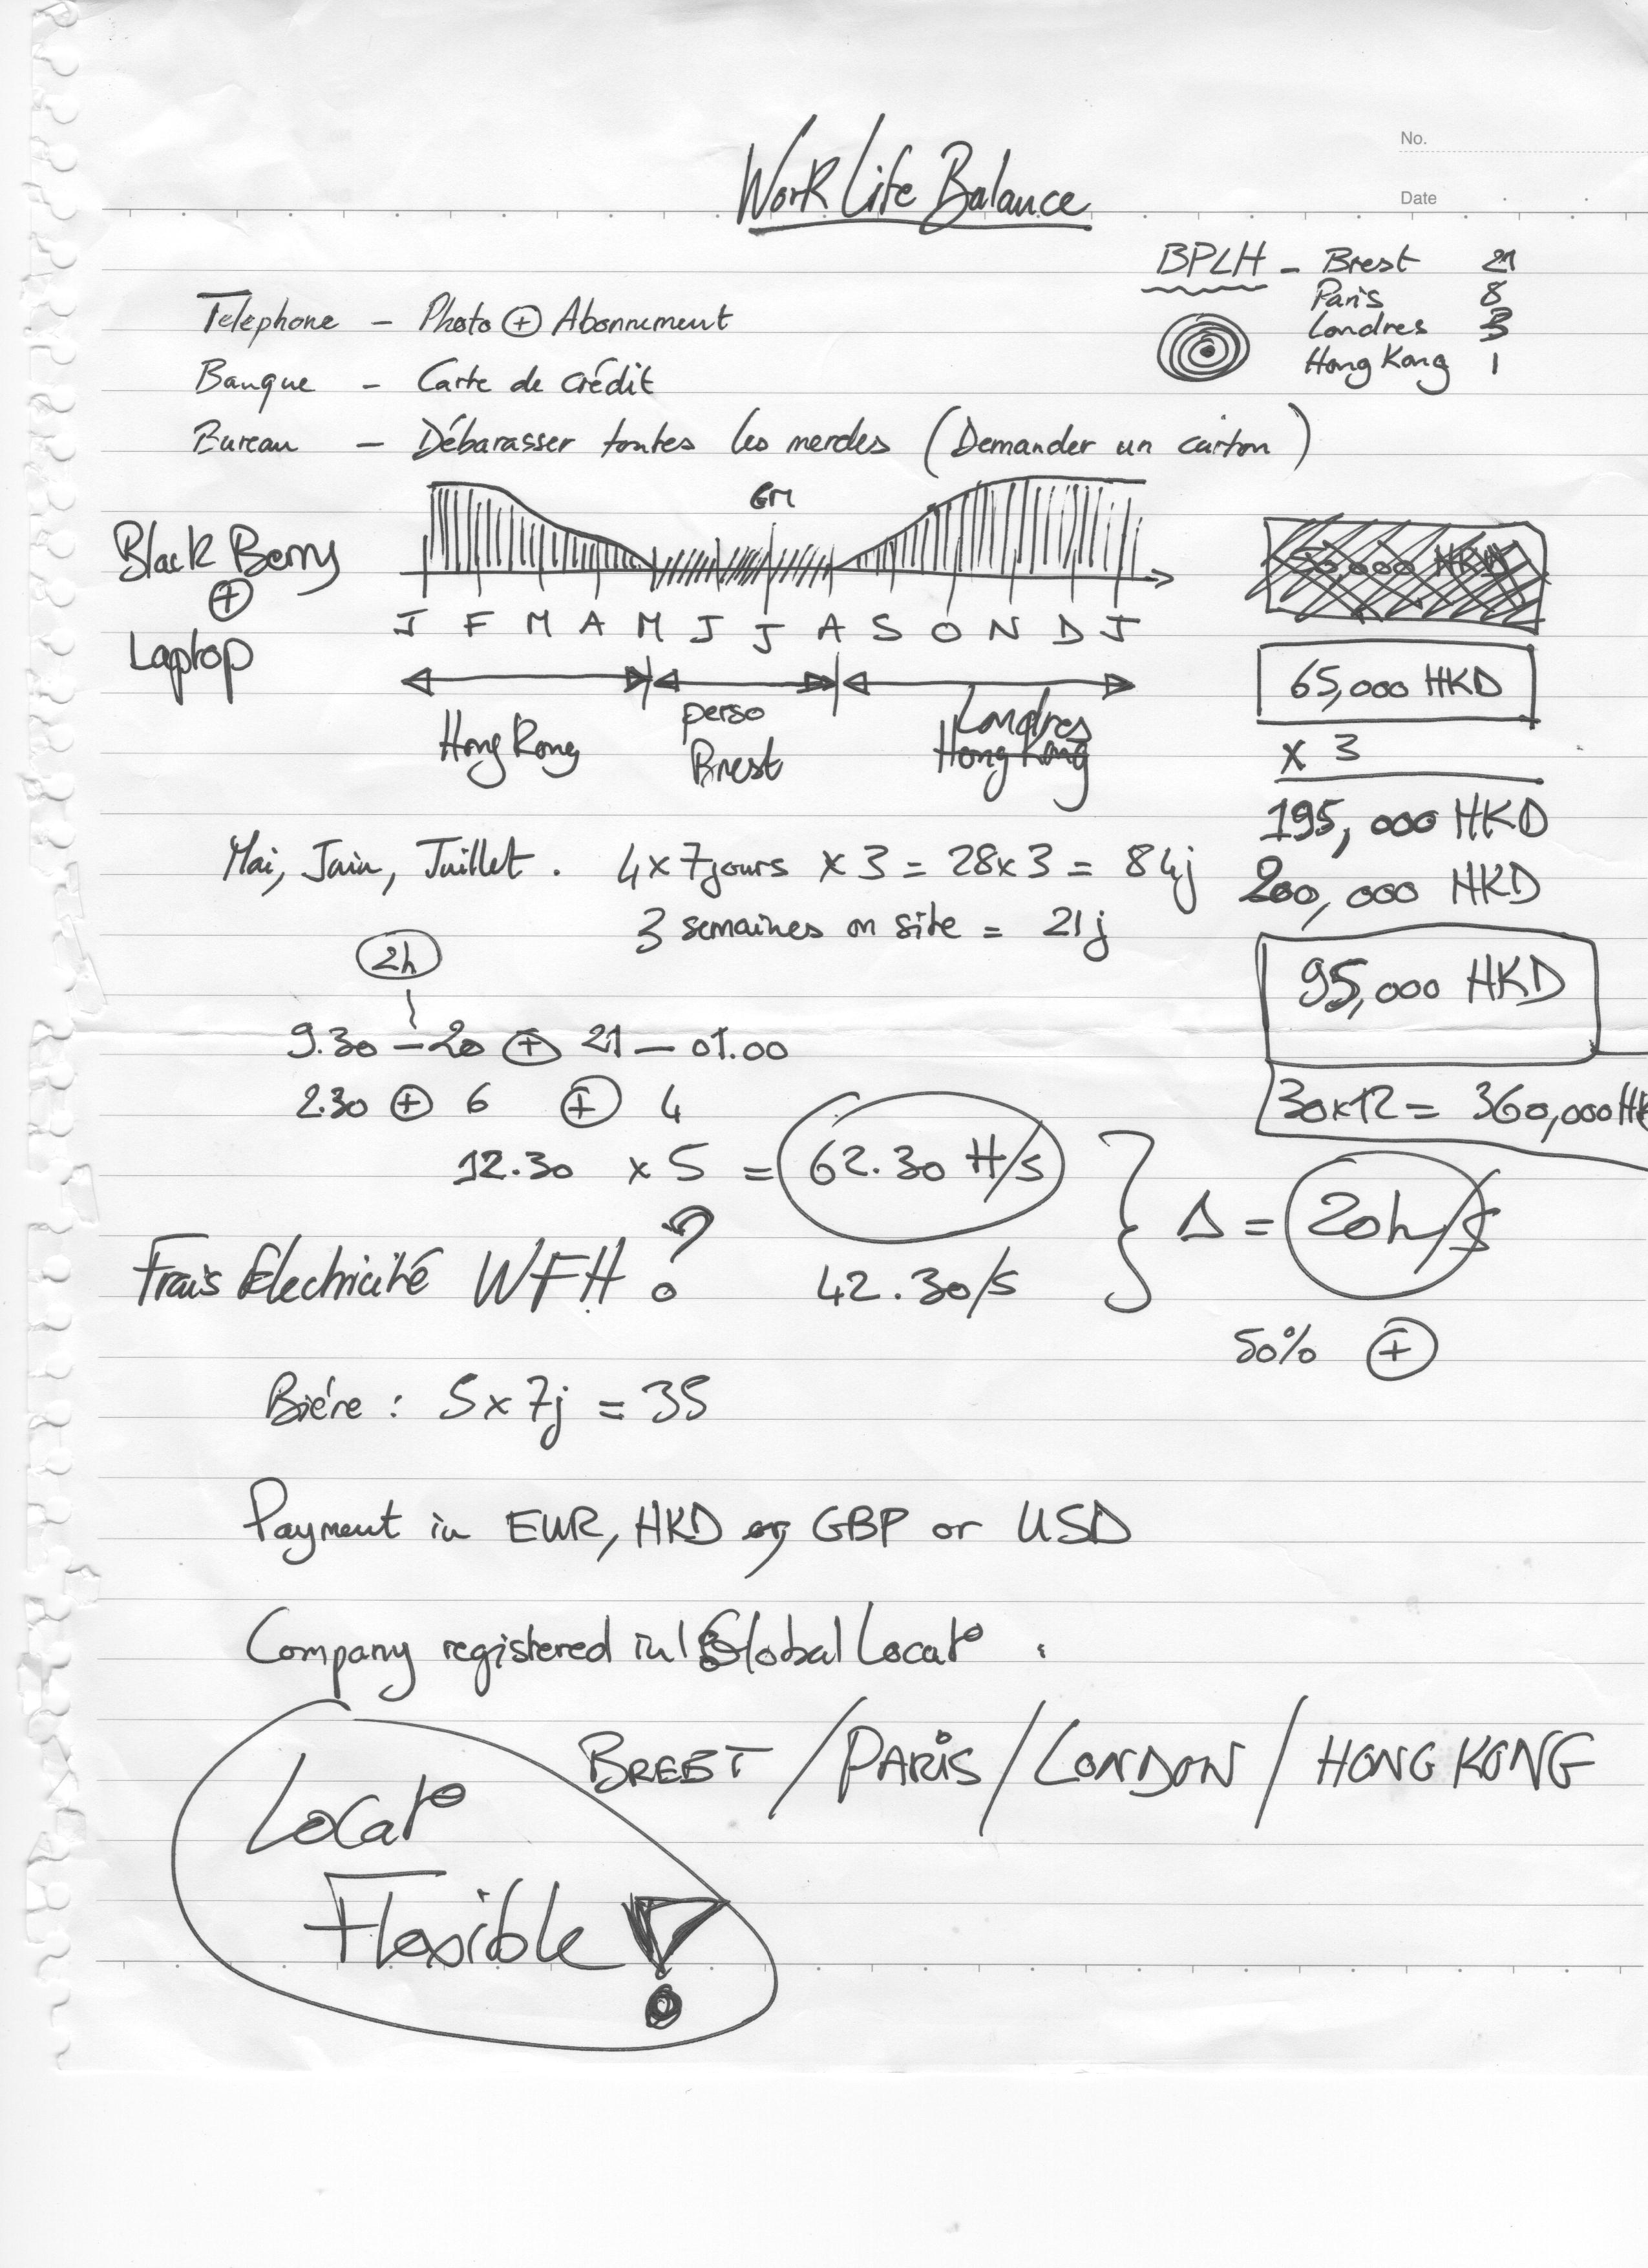
\includegraphics[width=200pts]{007.jpg}
\subsection{Gantt}
%#####################################################################################

\begin{figure}[ftbp]
\begin{center}

\begin{ganttchart}[y unit title=0.4cm,
y unit chart=0.5cm,
vgrid,hgrid, 
title label anchor/.style={below=-1.6ex},
title left shift=.05,
title right shift=-.05,
title height=1,
bar/.style={fill=gray!50},
incomplete/.style={fill=white},
progress label text={},
bar height=0.7,
group right shift=0,
group top shift=.6,
group height=.3,
group peaks={}{}{.2}]{24}
%labels
\gantttitle{Week}{24} \\
\gantttitle{Monday}{4} 
\gantttitle{Tuesday}{4} 
\gantttitle{Wednesday}{4} 
\gantttitle{Thursday}{4} 
\gantttitle{Friday}{4} 
\gantttitle{Saturday}{4} \\
%tasks
\ganttbar{first task}{1}{2} \\
\ganttbar{task 2}{3}{8} \\
\ganttbar{task 3}{9}{10} \\
\ganttbar{task 4}{11}{15} \\
\ganttbar[progress=33]{task 5}{20}{22} \\
\ganttbar{task 6}{18}{19} \\
\ganttbar{task 7}{16}{18} \\
\ganttbar[progress=0]{task 8}{21}{24}

%relations 
\ganttlink{elem0}{elem1} 
\ganttlink{elem0}{elem3} 
\ganttlink{elem1}{elem2} 
\ganttlink{elem3}{elem4} 
\ganttlink{elem1}{elem5} 
\ganttlink{elem3}{elem5} 
\ganttlink{elem2}{elem6} 
\ganttlink{elem3}{elem6} 
\ganttlink{elem5}{elem7} 
\end{ganttchart}
\end{center}
\caption{Gantt Chart}
\end{figure}
%#####################################################################################

\subsection{Resources}
Diagramme en etoile\\

\subsection{Burn down}
Graphique\\
Calcul de vitesse\\
Projection lineaire\\
Specialist tasks\\
Theoretical end\\

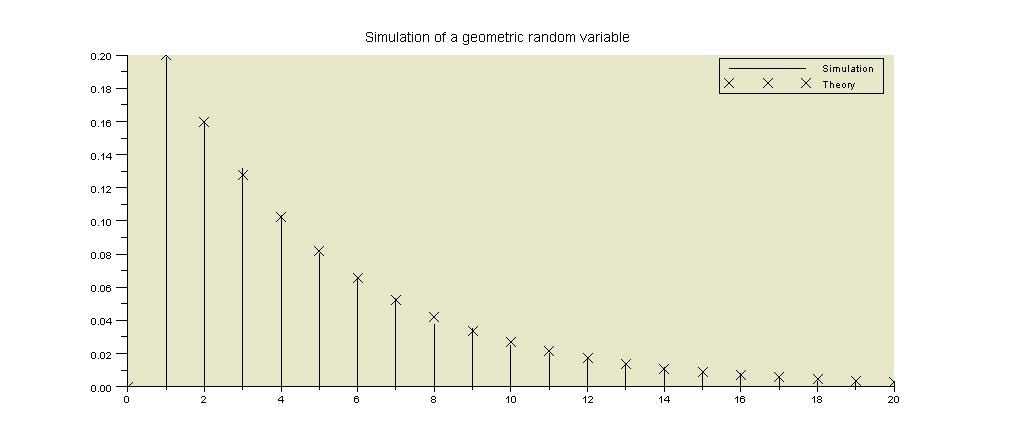
\includegraphics[width=200pts]{Geometric.jpg}

\subsection{Tasks}
List\\
Priorities\\
Cost \\
Dependances\\

\subsection{Risks}
Risk factors\\

\section{Research documents}

\subsection{FX vanilla}
Currency swap\\
FX Spot\\

\subsection{Fx Options}
Simple european pricing\\

\footnote{footnote text}

\subsection{Siv}
Monte Carlo simulation\\

\subsection{Fixed income}
Bond pricing\\

\subsection{IR derivatives}
Amortized swaps\\

\subsection{Equities}
Warrants\\
Vanilla option\\
Stock\\

\subsection{Credit}
CDOs\\
CDSindex\\
CDSbasket\\
Square CDOs

\subsection{Meetings}
Team meeting - Daily\\
Steering comittee - Bi weekly\\
Council - Monthly\\

\subsection{Sponsors}
Front office\\
IT\\
Risk management\\
CA\\
HSBC\\

\subsection{Stakeholders}
Front Office : Thibauld Deroux\\
IT : Andrew Jameson\\
Risk management : Axel Brabant\\


\end{document}
